% Section 4
\section{Extending BOSS: voBOSS and rBOSS}

\begin{frame}
\begin{center}
\textbf{Where can we go from here?}	
\end{center}

\end{frame}


\begin{frame}
\frametitle{We cannot know the best choice of k a priori}
As seen before construction and navigation of the graph was a space and time bottleneck when acting naively. \\
But we saw how to solve it using compression techniques
\\ \medskip 
Another problem emerges from the fact that state-of-the-art assemblers need to build the de Bruijn graph for multiple values
of K to obtain better sequencing results
\end{frame}


\begin{frame}
\frametitle{The need of the the right k}
\begin{columns}
	\column{0.5\textwidth}
	
	\textbf{Lower k}
	\begin{itemize}
		\item More connections
		\item Less chance of resolving small repeats
		\item Higher k-mer coverage
    \end{itemize}
	\textbf{Higher k}
	\begin{itemize}
		\item Less connections
		\item resolve small repeats
		\item Lower k-mer coverage
	\end{itemize}
	\column{0.5\textwidth}
	\begin{figure}	
		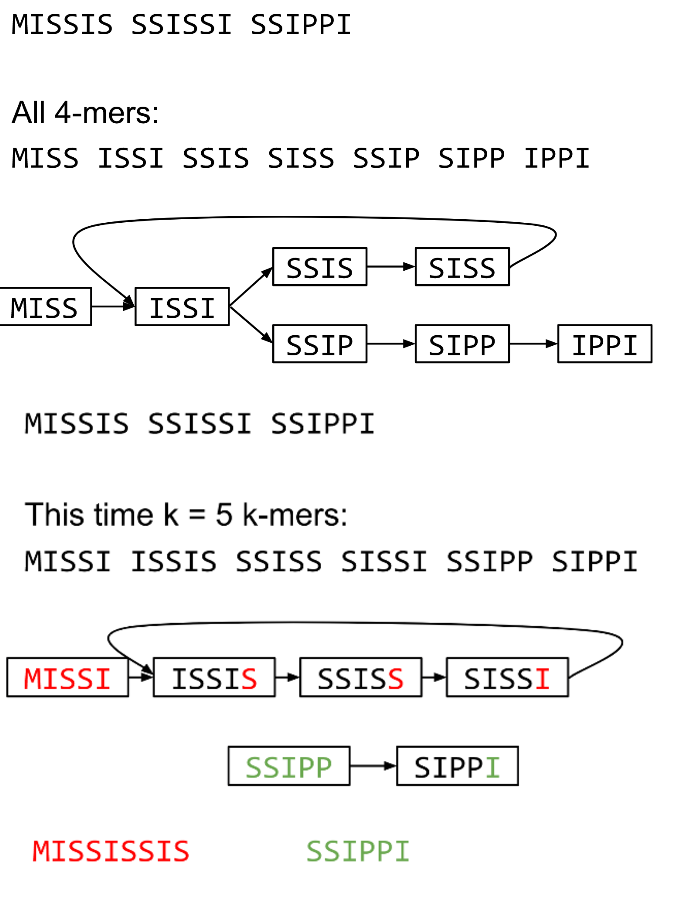
\includegraphics[height=1\textwidth,width=0.8\textwidth]{img/merged-dbg.png}
	\end{figure}
\end{columns}
\end{frame}


\begin{frame}
\frametitle{Variable order dBG (Gagie et al., 2014)}
In 2014 Gagie et al. showed how to augment a succinct de Bruijn graph
representation letting us change order on the fly.
% effectively representing all de Bruijn graphs of order up to some maximum K in a single data structure.
\\ \medskip
Just following a simple observation: deleting the first column of the BOSS-matrix the result is almost the BOSS matrix for a 2nd-order de Bruijn graph.
\\ \medskip
This truncated form of a higher order BOSS differs from the BOSS of a lower order in that some rows are repeated
\\ \medskip
This fact could prevent the BOSS representation from working properly. 
\end{frame}

\begin{frame}
\frametitle{Fixing it}
Instead of trying to apply forward, backward and
lastchar directly to nodes in the lower-order-graphs, we augment the BOSS representation of
the original graph to support the following three queries:
\begin{itemize}
	\item \textbf{shorter(v, k)} returns the node whose label is the last k characters of v’s label;
	\item \textbf{longer(v, k)} lists nodes whose labels have length k ≤ K and end with v’s label;
	\item \textbf{maxlen(v, a)} returns some node in the original graph whose label ends with v’s. label, and that has an outgoing edge labelled a, or NULL otherwise.
\end{itemize}
\end{frame}


\begin{frame}
\frametitle{}
If v is a node in the original graph then we
can use the BOSS implementations of forward, backward and lastchar.
\\ \medskip
Otherwise, if v’s label has length $k_v \leq k$ then:
\begin{itemize}
	\item \textbf{fwd(v, a) = shorter(fwd(maxlen(v, a), a), $k_v$ )}
	\item \textbf{bwd(v) = shorter(bwd(maxlen(longer(v,$k_v$+ 1), ∗)), $k_v$ )}
	\item \textbf{lastchar(maxlen(v, ∗))}
\end{itemize}
\end{frame}


\begin{frame}
\frametitle{Implementing shorter and longer}
To implement shorter and longer, we store a wavelet tree over the sequence $L^∗$
in which $L^* [i]$ is the length of the longest common suffix of Node[i] and Node[i+1].
\\ \medskip
This takes $\mathcal{O}(log\ K)$ bits per (K + 1)-tuple in the matrix.\\
To save space, we can omit Ks in $L^∗$, since they correspond to 0s in L and indicate that Node[i] and Node[i+1] are in the interval of the same node in the original graph;
\\ \medskip 
the wavelet tree then takes $\mathcal{O}(log\ K)$ bits per node in the original graph and $\mathcal{O}(n\ log\ K)$  bits in total.
\\ \medskip
In our example, $L^∗ = [0, 1, 0, 3, 2, 1, 0, 3, 2, 0, 1, 1 ]$
(we can omit the 3s to save space).
\end{frame}


\begin{frame}
\frametitle{Conclusions: Versatility of BOSS}
The goodness of the BOSS representation was highlighted both by the original results and by all the extensions that came out in the following years.
\\ \medskip
Infact we just saw how to use BOSS to deal with variable order de Bruijn graphs.
\\ \medskip
But the improvements are not over ...
\end{frame}


\begin{frame}
\frametitle{Concluding: simulating the overlap graph}
In 2019 Dominguez et al [3] showed that BOSS can be extended even more arriving to simulate the overlap graph on the fly
\\ \medskip
The authors observed that overlaps between reads can be computed using voBOSS
\end{frame}

\begin{frame}
\frametitle{Link between variable-order and overlaps}
- extend a unary path using solid nodes as much as possible; 
\\ \medskip
- if a solid node v without outgoing edges is reached, then decrease its order with shorter to retrieve the nodes that represent both a suffix of v and a prefix of some other read.
\\ \medskip
- from these nodes, retrieve the overlapping solid nodes of v by using forward and continue the graph right traversal from one of them.
\end{frame}

\begin{frame}
\frametitle{When does shorter work correctly?}
Since shorter does not ensure that the label of the output node appears as a prefix in the set of reads we need some precise conditions:
\begin{lemma}
	In voBOSS, applying the operation shorter to a node v of order $k' \leq k$ will
	return a node u of order $k'' < k'$ that encodes a forward overlap for v \\
	$\Leftrightarrow$\\
	u[1] is a linker node contained by v.
\end{lemma}
\end{frame}

\begin{frame}
\frametitle{rBOSS fundamentals}
We are ready to define the two operations needed to compute overlaps using voBOSS:
\begin{itemize}
	\item \textbf{nextcontained(v)}: returns the greatest linker node v , in lexicographical order, whose llabel represents both a suffix of v and a prefix of some other node in G.
	\item \textbf{buildL(v,m)}: returns the set of all the linker nodes contained by v that represent a suffix of v
	of length $\geq m$.
\end{itemize}
the second operation is needed since a node might have more than one contained linker node, and those linkers whose \textbf{llabel} is of length $\geq m$ represent edges in the overlap graph.
\end{frame}

\begin{frame}
\frametitle{Final remarks}
\begin{itemize}
	\item if we chose $k = z + 1$ to build voBOSS we are simulating the full overlap graph in compressed space.\\
	The edges are not stored explicitly, but computed on the
	fly by first obtaining L = buildL(v, m), and then following the dBG outgoing edges of every l ∈ L.
	\item This extension substitutes the \textbf{LCS} over \textbf{L} with a compacted trie to achieve fast implementation of \textbf{buildL(v,m)}.
	
\end{itemize}

\end{frame}

